
\part{Einleitung}
%----------------------------------------------------------------------------------------
%	CHAPTER 1
%----------------------------------------------------------------------------------------
\chapterimage{Bilder_und_Co/ai_safety_landscape.png} % Chapter heading image
%----------------------------------------------------------------------------------------

\chapter{Aufgabenstellung}
Mit dem zunehmenden Einsatz \ac{KI} in sicherheitskritischen Bereichen wie der Luftfahrt gewinnt die Frage nach der Verlässlichkeit, Transparenz und Absicherung solcher Systeme zunehmend an Bedeutung. Ziel dieser Bachelorarbeit ist es, existierende Konzepte und Methoden zur Sicherheit von KI-Systemen (AI Safety) systematisch zu untersuchen und im Hinblick auf ihre potenzielle Anwendbarkeit in luftfahrttechnischen Radarsystemen zu analysieren. Dabei soll herausgearbeitet werden, welche spezifischen Herausforderungen sich bei der Übertragung solcher Methoden auf Radarsysteme ergeben, und inwieweit bestehende Sicherheitsansätze – insbesondere unter Berücksichtigung der Norm ISO 8800 – diesen Anforderungen gerecht werden können.

Im Rahmen der Arbeit ist zunächst eine fundierte Literaturrecherche durchzuführen, um die relevanten Begriffe und Themenfelder – insbesondere Künstliche Intelligenz, Radartechnologie und Sicherheit – einzuordnen und abzugrenzen. Darauf aufbauend sollen gängige KI-Modelle sowie typische Einsatzszenarien von Radarsystemen in der Luftfahrt beschrieben und analysiert werden. Weiterhin sind bestehende AI-Safety-Methoden hinsichtlich Transparenz, Robustheit und Fehlervermeidung zu untersuchen und auf ihre Übertragbarkeit auf sicherheitsrelevante luftfahrttechnische Anwendungen zu bewerten. Ein besonderer Fokus liegt dabei auf der Norm ISO 8800: Es soll analysiert werden, welche Anforderungen sie an KI-Systeme stellt, welche Probleme sie adressiert und inwiefern ihre Inhalte auf Anwendungen in der Luftfahrt übertragbar sind.

Darüber hinaus sollen reale Anwendungsbeispiele, Problemmeldungen oder Vorfälle im Zusammenhang mit dem Einsatz von \ac{KI} in sicherheitskritischen Systemen gesammelt und ausgewertet werden, um potenzielle Risiken und Schwachstellen zu identifizieren. Die Arbeit soll zudem die Möglichkeit eines konkreten Use Cases für KI-gestützte Radarsysteme aufzeigen und im Rahmen einer qualitativen Kosten-Nutzen-Betrachtung die Vorteile und potenziellen Gefahren des KI-Einsatzes gegeneinander abwägen. Abschließend sind konkrete Empfehlungen für die Anwendung von AI-Safety-Maßnahmen in der Luftfahrt abzuleiten. 

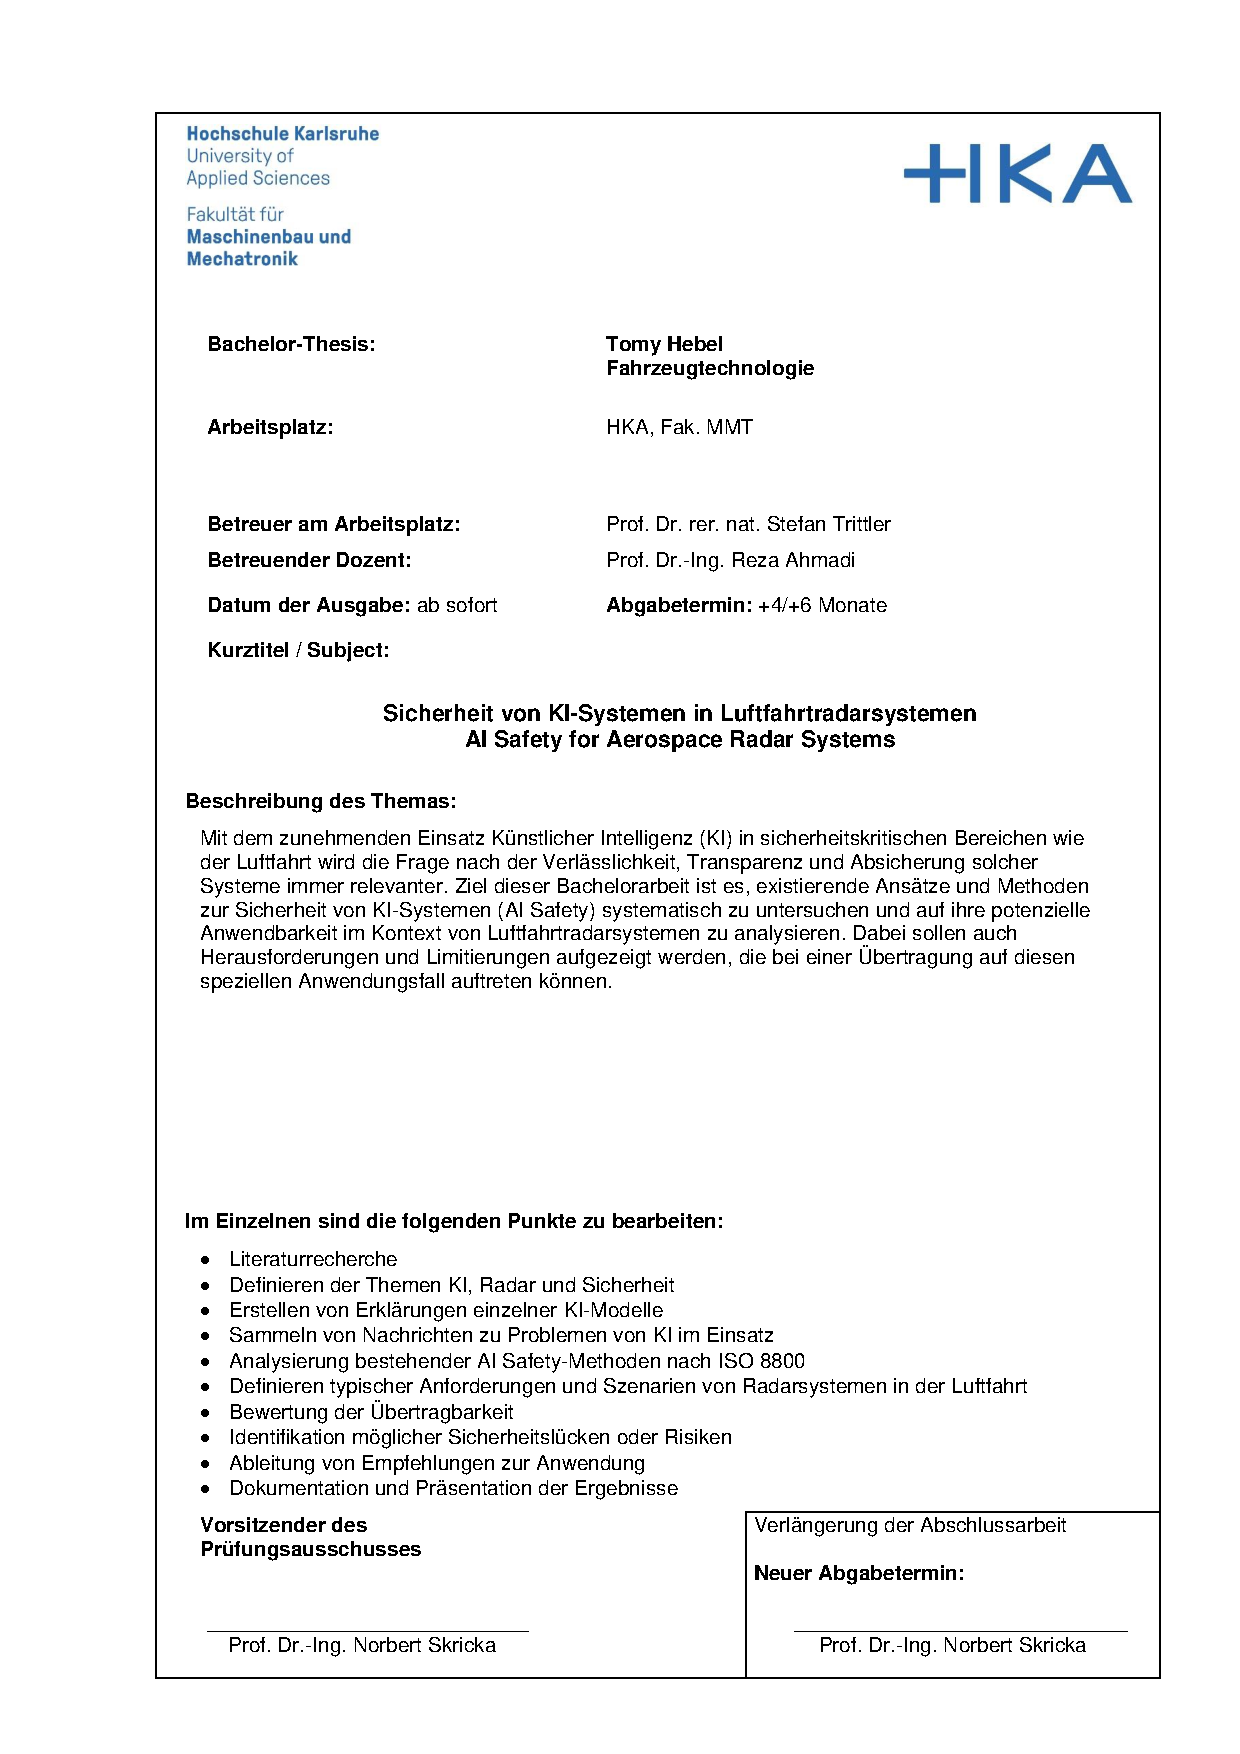
\includepdf[fitpaper=true, pages=-]{Bilder_und_Co/Sicherheit von KI-Systemen in Luftfahrtradarsystemen(1).pdf}

\chapter{Motivation und Ziel der Projektes}
Mit dem immer weiter verbreiteten Einsatz und Akzeptanz von \ac{KI} stellt sich die Frage, 
ob diese auch in der Luftfahrt Anwendung finden kann. Um diese Frage beantworten zu können, 
müssen \ac{KI} Modelle und ihr Eisatzgebiet auf Sicherheit überprüft werden. 

Ziel der Arbeit ist es, anhand des Beispieles von Radarsystemen zu überprüfen, 
ob KI-Systeme mittels bekannter Methodiken diese auf Sicherheit zu überprüfen ob sie den Anforderungen entsprechen, 
um diese in der Luftfahrt verwenden zu können.

\section{Weiteres}
In verschiedenen Paper wird gezeigt, dass \ac{KI} bei Radarsystemen was die Perfomance angeht, mit herkömmlichen Methoden 
mindestens mithalten kann oder diese was Rechenleistung, Speicher und Genauigkeit von Objekterkennung übertrifft. 
Dies unterstreicht weiter, dass es sehr nützlich sein kann \ac{KI} in diesem Feld zu benutzen. Doch in der Luftfahrt ist 
Sicherheit von großer Bedeutung und die meisten Paper die bei der Recherche zu diesem Thema gefunden wurden gehen 
auf die Performance der untersuchten KIs ein und untersuchen diese nicht auf Sicherheit, dies zeigt nochmals deutlich die Bedeutung 
dieser Arbeit. Doch was bedeutet sichere \ac{KI}? Ein Beispiel für eine Anforderung für eine sichere Software kann sein, 
dass diese deterministisch sein soll. Doch dies ist bezogen auf KIs problematisch umzusetzen, eine Möglichkeit wäre es, 
alle Möglichen Inputs und deren Outputs zu untersuchen bevor man die \ac{KI} verwendet. Aber das funktioniert nur bei 
kleieneren Modellen und würde vorallem bei Foundation Models einen zu großen Rechenaufwand bedeuten, als dass diese Methode 
verwendet werden könnte. Hier wäre eine persöhliche Idee einen Markowschen ansatz zu versuchen...??

\chapter{Hypothese}

\chapter{Methodisches Vorgehen}
\section{Besonders wichtige Literatur}
Zunächst wurde mit Absprache des Betreuenden Professors und dem Zweitkorrektor, eine kurze Liste an 
"Goldstandard-" Literatur festgelegt. Diese umfasst die recht neu erschienene ISO 8800 aus der Automobilbranche, 
welche die KI-Sicherheit in der Automobilbranche definiert. Die DO 178C weche über die Sicherheit von geschriebenen 
Computer Code in der Luftfahrt handelt. Und zum Schluss die EASA Roadmap und Concept Paper, welche beschreiben sollen, 
wie die Adaption von KI in der Luftfahrtbranche von statten gehen soll.


ISO 8800:

Diese ist die nach eigener Einschätzung, die derzeit Wertvollste Norm im Bezug auf KI-Sicherheit passend zum Kontext. 
Das liegt unteranderem an der Verwandschaft von der Luftfahrt und Automobilbranche, einerseitz technisch bzw. welche 
Ingenieurs-Fachgebiete abgedeckt werden, sowohl bei einem Flugzeug als auch bei einem Fahrzeug z.B. Aerodynamik, Elektrotechnik, 
Programmieren und vieles mehr. Die größeren Unterschiede hier liegen daher eher in den Anforderungen und Herangehensweisen 
im Bezug zur Sicherheit. Um beispielhafft einen sehr deutlichen Unterschied zu nennen, gibt es in der Automobilbranche 
die ISO 26262, die SOTIF Norm, welche sich mit der Sicherheit der Fuktionalität, unteranderem auch während des Betriebs 
des Fahrzeugs beschäftigt. Das kann zufolge haben, dass später im Lebenszyklus z.B. Softwareupdates erforderlich sind. 
Im Gegensatz wird in der Luftfahrt dieses Thema hauptsächlich im Frontloading behandelt, unter der Prämisse, dass das Flugzeug 
bereits bei erstigem Einsatz alle Sicherheitsanforderungen zur Gänze erfüllt und spätere Softwareupdates obsulet macht oder 
vorher definiert wird was und wann geändert werden muss mittels Updates.

Des Weiteren ähneln sich beide Branchen im Bezug auf die Sicherheit einzelner Komponenten. Z.B. werden in der Automobilbranche 
sehr hohe Sicherheitsanforderungen für einzelne Komponenten definiert, damit diese nicht redundant verbaut werden müssen und somit 
der Stückpreis pro Fahrzeug steigt, da bei Großserien redundante Teile sehr teuer sind. Hingegen wird in der Luftfahrt 
allgemein sehr hohe Ansprüche an alle einzelnen Teile gelegt, da die Gefahr bei Fehlfunktionen in einem Flugzeug sehr schnell 
lebensbedrohlich wird. Um weitere Sicherheit zu gewährleisten und um die definierten Anforderungen zu erfüllen werden die 
Teile in einem Flugzeug redundant verbaut.

Weitere Technische Unterschiede der Branchen gehen aus ihrer Natur herfor. In der Automobilbranche wird sehr viel B2C gehandelt, 
während die Luftfahrt hauptsächlich B2B handelt. Aufgrund der im Vergleich geringeren Lebensbedrohlichkeit bei Fehlfunktionen 
und der Branchennatur private Kunden zu gewinnen, befasst sich die Automobilbranche unteranderem viel mit technischen Begeisterungsmerkmahlen. 
Die Luftfahrt verfolgt das Ziel Geschäftskunden zu gewinnen, welche andere Wünsche haben als Privatpersonen.
Auf Grund dieses Unterschiedes kann sich die Automobilbranche sehr früh mit neueren Technologien auseinandersetzen, wo hingegen die 
Luftfahrt sich intensiv mit der Notwendigkeit und Sicherheit dieser neuen Technologien befasst. Weiter zu betrachten ist der gesammte Produktlebenszyklus, 
da Flugzeuge ca. zweimal so lange im Gebrauch sind wie Autos, was das Thema Sicherheit verkompliziert, besonders unter der Berücksichtigung 
von sich verändernde Umgebungen. (Beispiele hierfür sind im Straßenverkehr in den letzten Jahren eine größere Verbreitung von 
Elektrorollern zu beobachten. Und in der Luftfahrt nimmt der Einsatz von Dronen zu.)Z.B. kann die Automobilbranche mit einer KI 
gesteuerten Schilderkennung Kundengewinnen und Erfahrungen sammeln, während in der Luffahrt Wolken und Wetter Erkennung mit einer 
KI die Evaluierung und Entwicklung langwieriger ist. Das und noch mehr Gründe erklären, warum 
es die Luftfahrbranche daher technologisch träger macht. Aufgrund dieser Natur und der technischen Verwandheit wäre es sinnvoll, 
dass die Luftfahrt von den Erfahrungen der Automobilbranche lernen kann.


DO 178C:

Diese Luftfahrt Norm befasst sich mit der Sicherheit von geschrieben Computercode, zu erwähnen sind die Normen, auf die Bezug genommen werden in der 
DO 178C. Z.B. die DO 330 und die DO 333, welche sich mit Sofwarewerzeugen und deren Zertifizierung beschäftigen. Um den Aufwand nicht in das Unermessliche 
zu treiben werden diese nur bei bedarf angeschnitten. Da KI in verschiedener Literatur beschrieben "(z.b. ISO 5469TR)" als mathematischer 
Algorithmus und Teil der Softeware behandelt werden kann/sollte muss KI auch in Einklang gebracht werden mit der DO 178C. Was hier besonders interessant 
ist, sind bestimmte Anforderungen an Computer Code. Z.B. das der Code deterministisch sein soll und eine MC/DC coverage. Das KI oftmals nicht deterministisch 
ist, ist Allgemeinwissen. "(Unter bestimmten Vorraussetzungen kann KI deterministisch sein, z.B. wenn man die Temperatur des Outputvektors in einem NN auf 0 setzt 
und man den gesammten Inputraum abgedeckt/getestet hat. Doch das ist meistens technisch nicht umsetzbar oder würde die Funktion/Fähigkeit der KI zusehr einschränken)" 
MC/DC coverage beschreibt, dass jede einzelne Bedingung bei Entscheidungen z.B. if/else Schleifen im Code auch stehts ein anderen Output erzeugt. 
Das eine KI diese Anforderung nicht erfüllen kann sollte ebenfalls recht offensichtlich sein. Doch das interessante ist, dass in der 
DO 178C das nur implizit und nicht explizit gefordert wird. Um etwas genauer zu werden, werden diese Anforderungen sowohl in der DO 178C als auch 330 und 333 sehr 
empfohlen und als "best practise" beschrieben.


EASA AI Roadmap:

Die EASA ist die Europäische Agentur für Flugsicherheit. Die Regularien der EASA werden weltweit als "best practise" Standards anerkannt.
Und um Produkte in der europäischen Luftfahrtbranche anbieten zu können, müssen Flugzeughersteller EASA-Zulassungen besitzen. 
Auf Grund dieser Bedeutung und des Wissens und Erfahrungen der Sicherheitsingenieure dieser Agentur, muss nicht weiter 
ausgeführt werden, warum diese veröffentlichten Konzepte hier mit besonderer Bedeutung berücksichtigt wurden.
Doch leider sind die Veröffentlichten Konzepte leider nicht mehr als genau das. In diesen Konzepten stehen 
viele "best practise" Methoden und zu berücksichtigende Punkte, jedoch leider nicht, wie bei einer Norm, 
dass wenn alle dieser Punkte erfüllt sind, dass das Produkt sicher ist. Hier ein kleiner Spoiler vorab, sehr viele dieser Punkte 
und Methoden sind deckungsgleich mit dem was in der ISO 8800 steht. Die ISO 8800 geht konkreter auf Anpassungen 
zu berücksichtigender Normen ein und beschreibt ins Detail was wie Dokumentiert werden muss. "(Weiteres später)"

\section{Recherche}
Der zweite Schritt war weitere Literaturrecherche. Für die vorliegende Recherche wurden verschiedene wissenschaftliche Quellen systematisch ausgewertet. 
Dabei kamen unter anderem etablierte Datenbanken wie Google Scholar, ProQuest und IEEE Xplore zum Einsatz. 
Zur Sicherstellung einer umfassenden Betrachtung des Themas wurde die Auswahl der Quellen jedoch nicht 
ausschließlich auf diese Datenbanken beschränkt, sondern durch weitere spezialisierte Plattformen und 
einschlägige Fachpublikationen ergänzt. Ziel war es, eine breite und ausgewogene Grundlage für die Analyse 
und Darstellung der Thematik zu schaffen. Zudem war das Vorgehen zuerst anhand des Titels eine Thematische 
Verwandschaft festzustellen. Wenn im Titel kein Hinweis auf eines der Subthemen: KI, Radarsysteme, Luftfahrt 
oder Sicherheit zu erkennen war, wurden die Wissenschaftlichen Paper nicht weiter evaluiert. Die Paper, 
die ein Hinweis auf mindestens eines dieser Subthemen aufwieß wurde es Systematisch festgehalten und anhand 
des Abstractes auf tiefergehende Relevanz untersucht. Wenn das Abstract weitere Thematische Zusammenhänge 
gezeigt hat, wurde es berücksichtigt. Probleme die hier öfter aufgetreten sind waren, dass im Kontext KI 
es sich oftmals um Performance Paper gehandelt hat. Diese Performance Paper folgten meist dem Schema zu erklären, 
wie, warum und wofür diese KI trainiert wurde und ihre Fähigkeiten aufgezeigt. Diese Paper hatten zwei Probleme, 
einerseits waren sie nicht besonders relevant für das Thema und eine relative Performance im Vergleich zu 
herkömmlichen Methoden wurde meist auch nicht ausgeführt.


\chapter{Aufbau der Arbeit}